\documentclass[mathserif,compress]{beamer} 

\usepackage{beamerthemeDresden} 
\usepackage[english]{babel}
\usepackage{amsmath,amssymb}
\usepackage[latin1]{inputenc}
\usepackage{palatino}
\usepackage{graphicx}
\usepackage{subfigure}
\usepackage{pgf}
\usepackage{relsize}
\beamertemplateshadingbackground{red!1}{blue!1}
% Use some nice templates
\beamertemplatetransparentcovereddynamic  
\usepackage{pgfpages} 

\def\beq{\begin{equation}}
\def\eeq{\end{equation}}
\def\bit{\begin{itemize}}
\def\eit{\end{itemize}}
\def\bdm{\begin{displaymath}}
\def\edm{\end{displaymath}}
\def\ben{\begin{enumerate}}
\def\een{\end{enumerate}}
\def\bc{\mathbf{c}}
\def\bh{\mathbf{h}}
\def\br{\mathbf{r}}
\def\bs{\mathbf{s}}
\def\bu{\mathbf{u}}
\def\bw{\mathbf{w}}
\def\bx{\mathbf{x}}
\def\by{\mathbf{y}}
\def\bz{\mathbf{z}}
\def\bA{\mathbf{A}}
\def\bD{\mathbf{D}}
\def\bG{\mathbf{G}}
\def\bI{\mathbf{I}}
\def\bQ{\mathbf{Q}}
\def\bR{\mathbf{R}}
\def\bS{\mathbf{S}}
\def\bV{\mathbf{V}}
\def\bW{\mathbf{W}}
\def\bX{\mathbf{X}}
\def\bY{\mathbf{Y}}
\def\bZ{\mathbf{Z}}
\def\cB{\mathcal{B}}
\def\cF{\mathcal{F}}
\def\cI{\mathcal{I}}
\def\cK{\mathcal{K}}
\def\cU{\mathcal{U}}
\def\bbeta{\mbox{\boldmath $\beta$}}
\def\bepsilon{\mbox{\boldmath $\epsilon$}}
\def\bdelta{\mbox{\boldmath $\delta$}}
\def\bgamma{\mbox{\boldmath $\gamma$}}
\def\bldeta{\mbox{\boldmath $\eta$}}
\def\bphi{\mbox{\boldmath $\phi$}}
\def\bkappa{\mbox{\boldmath $\kappa$}}
\def\blambda{\mbox{\boldmath $\lambda$}}
\def\bmu{\mbox{\boldmath $\mu$}}
\def\bnu{\mbox{\boldmath $\nu$}}
\def\btheta{\mbox{\boldmath $\theta$}}
\def\brho{\mbox{\boldmath $\rho$}}
\def\bDelta{\mbox{\boldmath $\Delta$}}
\def\bLambda{\mbox{\boldmath $\Lambda$}}
\def\bSigma{\mbox{\boldmath $\Sigma$}}
\def\var{\textrm{var}}
\def\cov{\textrm{cov}}
\def\log{\textrm{log}}
\def\median{\textrm{median}}
\def\argmin{\textrm{arg min }}
\def\bzero{\mathbf{0}}
\def\bone{\mathbf{1}}
\def\Poi{\textrm{Poi}}
\def\Unif{\textrm{Unif}}

%-------------------------------------------------------------------------------

\title[]{Estimating Abundance from Counts in Large Data Sets of Irregularly-Spaced Plots using Spatial Random Effects of Fixed Rank}

\author[Jay M. Ver Hoef]{Jay Ver Hoef} 

\institute[NOAA National Marine Mammal Lab]
{
	\normalsize NOAA National Marine Mammal Lab \\
	NOAA Fisheries \\
	International Arctic Research Center \\
	Fairbanks, Alaska, USA\\
	\vspace{0.1cm}
}
\date[06/22/10]{}
%-------------------------------------------------------------------------------
\begin{document}

%-------------------------------------------------------------------------------
\frame{\titlepage}
%-------------------------------------------------------------------------------

%-------------------------------------------------------------------------------
%                        OUTLINE
%-------------------------------------------------------------------------------

\section{Introduction}
\subsection{Outline}
\begin{frame} \frametitle{Outline}
     

	\begin{tabular} {p{5.8cm} p{3.8cm}}
	{
		\begin{center}
		\bit
			\item Introduction  \pause      
				\vspace{0.2cm}       
			\item Models  \pause         
				\vspace{0.2cm} 
			\item Inference  \pause    
				\vspace{0.2cm}      
			\item Simulations  \pause    
				\vspace{0.2cm}      
			\item Real Example \pause 
				\vspace{0.2cm}
			\item Summary
		\eit
	\end{center}
	} &
	{
		\vspace{-.5cm}
%		\hspace{-.7cm}
		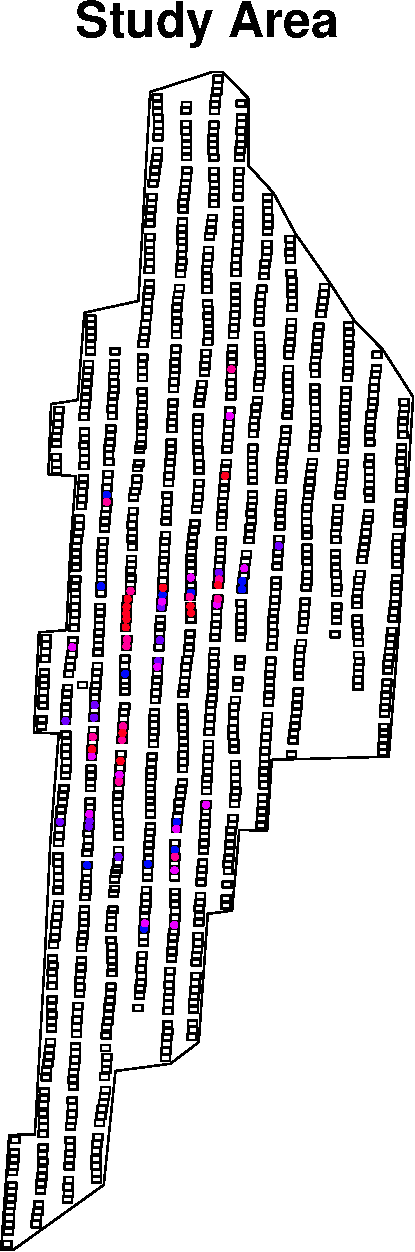
\includegraphics[width=2.0cm]{RawPlotsColoredCrop.pdf} 
	}
	\end{tabular}

\end{frame}
   
 
%-------------------------------------------------------------------------------
%                        Aerial Photos
%-------------------------------------------------------------------------------

\subsection{Aerial Photos}
\begin{frame} 
\frametitle{Aerial Photos}
     
	\begin{tabular} {p{5.8cm} p{3.8cm}}

		{
		\begin{center}
		  \vspace{-.5cm}
			\includegraphics[width=4.0cm]{airplane.jpeg}  \\
		  \vspace{.5cm}
			\includegraphics[width=4.0cm]{cameras.jpeg} \\
		\end{center}
		} &
		{
			\vspace{-.5cm}
			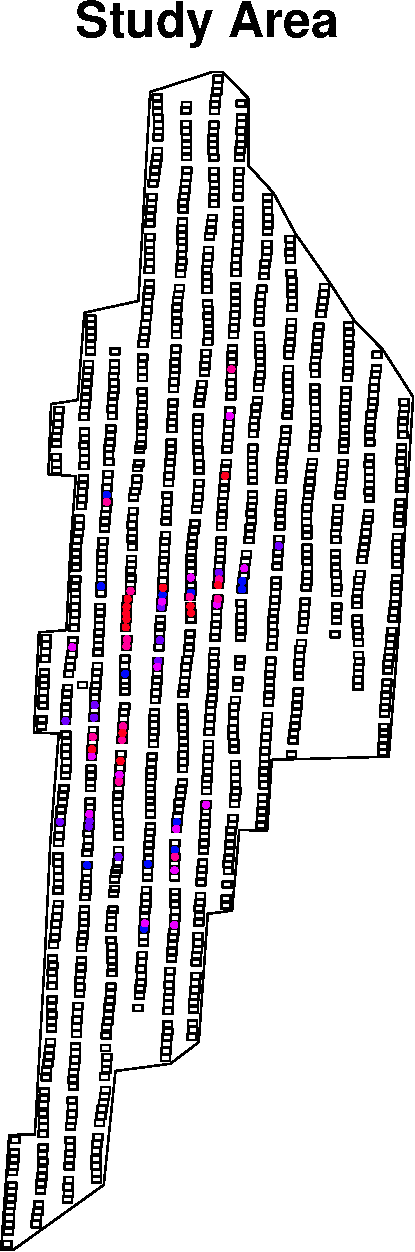
\includegraphics[width=2.0cm]{RawPlotsColoredCrop.pdf} 
		}

	\end{tabular}

\end{frame}

%-------------------------------------------------------------------------------
%                        Aerial Photos
%-------------------------------------------------------------------------------

\subsection{Aerial Photos}
\begin{frame} 
\frametitle{Aerial Photos}
     
	\begin{tabular} {p{5.8cm} p{3.8cm}}

		{
		\begin{center}
		  \vspace{-.5cm}
			\includegraphics[width=4.0cm]{aerialPhoto.jpeg}  \\
		  \vspace{.5cm}
			\includegraphics[width=4.0cm]{SealInWater.jpeg}  \\
		\end{center}
		} &
		{
			\vspace{-.5cm}
			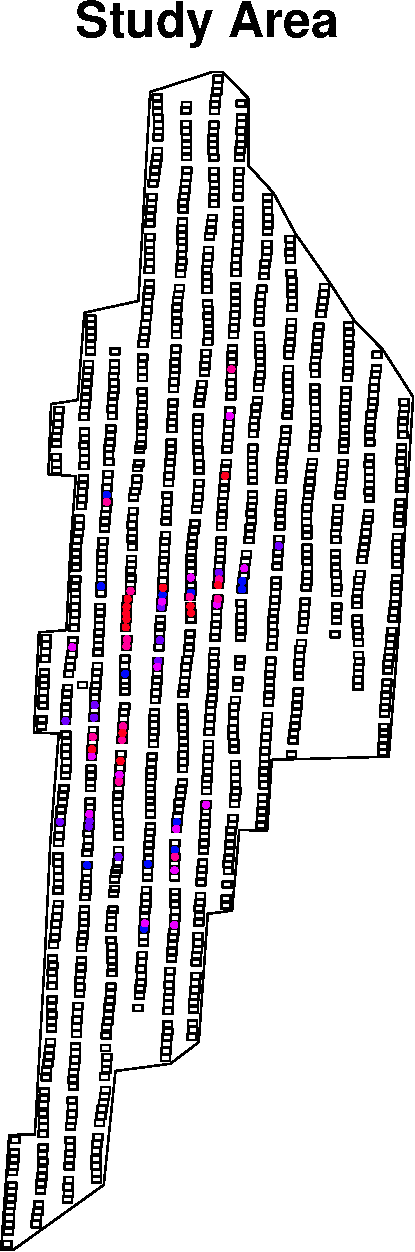
\includegraphics[width=2.0cm]{RawPlotsColoredCrop.pdf} 
		}

	\end{tabular}

\end{frame}
%-------------------------------------------------------------------------------
%                   INTRODUCTORY GRAPH
%-------------------------------------------------------------------------------

\subsection{Introduction}
\begin{frame}
\frametitle{Introduction}

	\begin{center} 
		\includegraphics[width=10cm]{FigRegionsSamples100925.pdf} 
	\end{center}

\end{frame}

%-------------------------------------------------------------------------------
%                   Inhomogeneous Point Process
%-------------------------------------------------------------------------------

\section{Models}
\subsection{Inhomogeneous Point Process}

\begin{frame}
\frametitle{Inhomogeneous Point Process}

	\centering
	{\color{blue} Intensity Function}
	\bdm
		\lambda(\bs) = \lim_{|dx| \to 0} \frac{E\left( T(dx) \right) }{|dx|} \hspace{.4cm}
		T(A) \textrm{: \# of events in } A
	\edm \pause
	{\color{blue} Expected Counts}
	\bdm
		\mu(A) = \int_A \lambda(\bu|\btheta) d\bu
	\edm \pause
	{\color{blue} Distribution}
	\bdm
		T(A) \sim \textrm{Poi}\left(\mu(A)\right)
	\edm
	\centering

\end{frame}

%-------------------------------------------------------------------------------
%                   Abundance Estimate
%-------------------------------------------------------------------------------

\subsection{Abundance Estimate}
\begin{frame}
\frametitle{Abundance Estimate}

	\centering
	\begin{tabular} {p{5.3cm} p{4.3cm}}
%	\vspace{-4cm}
	{
			\bdm
				\cB = \cup_{i = 1}^n B_i 
			\edm \pause
			\bdm
				\cU \equiv \overline{\cB} \cap A 
			\edm \pause
			\bdm
				\widehat{T}(A) = T(\cB) + \widehat{T}(\cU)
			\edm \pause
			\bdm
				\widehat{T}(\cU) = \hat{\mu}(\cU) = \int_\cU \hat{\lambda}(\bu|\btheta) d\bu
			\edm
			\bdm
				 = \int_\cU \lambda(\bu|\hat{\btheta}) d\bu
			\edm
	} &
	{
		\vspace{.5cm}
		\includegraphics[width=4.3cm]{Fig_RegionSamplesCrop.pdf} 
	}
	\end{tabular}
	\centering
\end{frame}

%-------------------------------------------------------------------------------
%                   Spatial Basis Functions
%-------------------------------------------------------------------------------

\subsection{Spatial Basis Functions}
\begin{frame}
\frametitle{Spatial Basis Functions}

\begin{tabular} {p{6.5cm} p{3.1cm}}
{
	$\by_1$,$\by_2$ jointly MVN,
	\bdm
		\cov\left(
		\begin{array}{c}
			\by_1 \\
			\by_2
		\end{array}
		\right) = \delta^2\left(
		\begin{array}{c c}
			\bV_{1,1} & \bV_{1,2} \\
			\bV_{1,2}^\prime & \bV_{2,2}
		\end{array} 
		\right)
	\edm \pause
	\bdm
		\rightarrow \cov(\by_1|\by_2) = \delta^2(\bV_{1,1} - \bV_{1,2}\bV_{2,2}^{-1}\bV_{1,2}^\prime)
	\edm \pause
	\bdm
		\textrm{Want } \sigma^2\bI = \delta^2(\bV_{1,1} - \bV_{1,2}\bV_{2,2}^{-1}\bV_{1,2}^\prime)
	\edm \pause
	\bdm
	\rightarrow \delta^2\bV_{1,1} =  \delta^2\bV_{1,2}\bV_{2,2}^{-1}\bV_{1,2}^\prime + \sigma^2\bI
	\edm
} & 
{
		\vspace{.5cm}
%		\hspace{.2cm}
		\includegraphics[width=3.09cm]{LocKnots.pdf} 
}
\end{tabular}

\end{frame}

%-------------------------------------------------------------------------------
%                   Spatial Basis Functions
%-------------------------------------------------------------------------------

\subsection{More Spatial Basis Functions}
\begin{frame}
\frametitle{More Spatial Basis Functions}

\begin{tabular} {p{6.2cm} p{3.7cm}}
{
	\bdm
		C(\bs_i,\bs_j) \equiv \cov(Z(\bs_i),Z(\bs_j)) 
	\edm \pause
	\bdm
		\bZ[i,j] = C(\bs_i,\bkappa_j)
	\edm \pause
	\bdm
		\bG[j,j^\prime] =  C(\bkappa_j,\bkappa_{j^\prime})
	\edm \pause
	\bdm
		\bG = \bQ\bLambda\bQ^\prime, \bQ^\prime\bQ = \bI
	\edm \pause
	\bdm
		\bZ_G \equiv \bZ\bQ\bLambda^{-1/2}
	\edm
} & 
{
		\vspace{.5cm}
%		\hspace{.2cm}
		\includegraphics[width=3.69cm]{LocKnots.pdf} 
}
\end{tabular}

\end{frame}

%-------------------------------------------------------------------------------
%           Linear Mixed Models with Spatial Basis Functions
%-------------------------------------------------------------------------------

\subsection{Linear Mixed Models with Spatial Basis Functions}
\begin{frame}
\frametitle{Linear Mixed Models with Spatial Basis Functions}

\begin{tabular} {p{6.2cm} p{3.7cm}}
{
	\bdm
		\bY = \bX\bbeta + \bZ_G\bgamma + \bepsilon 
	\edm
	$\cov(\bgamma) = \delta^2\bI, \; \cov(\bepsilon) = \sigma^2\bI$ \pause
	\bdm
		\cov(\bY) = \delta^2\bZ_G\bZ_G^\prime + \sigma^2\bI
	\edm \pause
	\bdm
		= \delta^2\bZ\bG^{-1}\bZ^\prime + \sigma^2\bI
	\edm \pause
	\bdm
		\left(\delta^2\bV_{1,2}\bV_{2,2}^{-1}\bV_{1,2}^\prime + \sigma^2\bI \right)
	\edm
} & 
{
		\vspace{.5cm}
		\includegraphics[width=3.69cm]{LocKnots.pdf} 
}
\end{tabular}

\end{frame}

%-------------------------------------------------------------------------------
%           Two Scales of Spatial Basis Functions
%-------------------------------------------------------------------------------

\subsection{Two Scales of Spatial Basis Functions}
\begin{frame}
\frametitle{Two Scales of Spatial Basis Functions}

\begin{tabular} {p{6.5cm} p{3.1cm}}
{
	\hspace{-.5cm}
	\bdm
			\cov(\bY) =
	\edm
	\bdm
		\begin{array} {c}
			{
				\left[ 
					\bZ_{G,C}|\bZ_{G,F}
				\right]
				\left[
					\begin{array} {c c}
						\delta_C^2\bI & \bzero  \\
						\bzero & \delta_F^2\bI
					\end{array}
				\right]
				\left[
					\begin{array} {c}
						\bZ_{G,C}^\prime \\
						\bZ_{G,F}^\prime
					\end{array} 
				\right] 
			} \\
			+ \sigma^2\bI
		\end{array}
	\edm \pause
	\bdm
		= \bW\bD\bW^\prime + \sigma^2\bI
	\edm \pause
	\bdm
		=\delta_C^2\bZ_C\bG_C^{-1}\bZ_C^\prime + \delta_F^2\bZ_F\bG_F^{-1}\bZ_F^\prime + \sigma^2\bI
	\edm
} & 
{
		\vspace{.5cm}
		\includegraphics[width=3.09cm]{Knots2Scales.pdf} 
}
\end{tabular}

\end{frame}

%-------------------------------------------------------------------------------
%           Intensity Surfaces to GLMMs
%-------------------------------------------------------------------------------

\subsection{Intensity Surfaces to GLMMs}
\begin{frame}
\frametitle{Intensity Surfaces to GLMMs}

	\bdm
		E[Y(B_i)] = \int_{B_i} \lambda(\bu|\btheta) d\bu
	\edm \pause
	\bdm
		\approx |B_i| \lambda(\bs_i|\btheta)
	\edm \pause
	\bdm
		Y_i \sim \Poi(|B_i| \lambda(\bs_i|\btheta))
	\edm \pause
	\bdm
		Y_i \sim \Poi\left( |B_i| \exp(\bX[i,\cdot]\bbeta + 
			\bZ_{G,C}[i,\cdot]\bgamma_C + \bZ_{G,F}[i,\cdot]\bgamma_F)\right)
	\edm \pause
	\bdm
		Y_i \sim \Poi\left(\exp(\beta_0 + 
			\bZ_{G,C}[i,\cdot]\bgamma_C + \bZ_{G,F}[i,\cdot]\bgamma_F)\right)
	\edm
	$\textrm{where } \btheta = [\beta_0, \bgamma, \delta_C^2, \delta_F^2]$

\end{frame}

%-------------------------------------------------------------------------------
%           Quasi-Models
%-------------------------------------------------------------------------------

\subsection{Quasi Mixed Models}
\begin{frame}
\frametitle{Quasi Mixed Models}
	\vspace{-.5cm}
	\bdm
		E(\bY|\bgamma) = g^{-1}(\bX\bbeta + \bW\bgamma) = 
		\exp(\bX\bbeta + \bW\bgamma) = \exp(\bldeta) = \bmu
	\edm 
	$\textrm{where } \bgamma \sim N(\bzero, \bD), 
		\var(\bY|\mbox{\boldmath $\gamma$}) = \bA$ \pause
	\bdm
		\tilde{\bY} = \bX\bbeta + \bW\bgamma + \bepsilon
	\edm \pause
	$\textrm{where }\tilde{\bY} = \tilde{\bDelta}^{-1}\left(\bY - 
	  g^{-1}(\bX\tilde{\bbeta} + \bW\tilde{\bgamma})\right) + 
	  \bX\tilde{\bbeta} + \bW\tilde{\bgamma}$
	\bdm
   \tilde{\bDelta} \equiv  
     \frac{\partial g^{-1}(\bldeta)} 
     {\partial \bldeta} = \exp(\bldeta)
	\edm \pause
	\bdm
   \textrm{var}(\bepsilon) =   
     \tilde{\bDelta}^{-1}\bA\tilde{\bDelta}^{-1} \equiv \tilde{\bA}	
	\edm \pause
	\bdm
		\var(\tilde{\bY}) =  \bW\bD\bW^\prime + 
    \tilde{\bA} \equiv \tilde{\bV}
	\edm

\end{frame}


%-------------------------------------------------------------------------------
%           Fitting Algorithm
%-------------------------------------------------------------------------------

\section{Inference}

\subsection{Fitting Algorithm (IWLS)}
\begin{frame} 
\frametitle{Fitting Algorithm (IWLS)}
     
	\begin{center}
	\bit
		\item Step 1.  Form pseudo-data $\tilde{\bY}^{[t+1]}$ using 
			\bdm
				\begin{array}{c}
				\tilde{\bY}^{[t+1]} = \tilde{\bDelta}^{-1}\left(\bY -
				\exp(\bX\tilde{\bbeta}^{[t]} + [\bZ_{G,C}|\bZ_{G,F}]\tilde{\bgamma}^{[t]})\right) + \\
				\bX\tilde{\bbeta}^{[t]}+ [\bZ_{G,C}|\bZ_{G,F}]\tilde{\bgamma}^{[t]}
				\end{array}
			\edm 
		with the current estimates $\tilde{\bbeta}^{[t]}$ and $\tilde{\bgamma}^{[t]}$ 
			for the $t$th iteration \pause
		\item Step 2.  Estimate $\hat{\delta}_C^{2[t+1]}$ and $\hat{\delta}_F^{2[t+1]}$ 
			as $\argmin l(\delta_C^2,\delta_F^2;\tilde{\bY}^{[t+1]})$ in 
			\bdm
				l(\delta_C^2,\delta_F^2;\tilde{\by}) = \log\left|\tilde{\bV}\right| +
				\br^{\prime}\tilde{\bV}^{-1}\br +
				\log\left|\bX^{\prime}\tilde{\bV}^{-1}\bX\right| + c
			\edm
	\eit
	\end{center}

\end{frame}

%-------------------------------------------------------------------------------
%           Fitting Algorithm
%-------------------------------------------------------------------------------

\subsection{Fitting Algorithm (IWLS)}
\begin{frame} 
\frametitle{Fitting Algorithm (IWLS)}
     
	\begin{center}
	\bit
		\item Step 3.  Using $\tilde{\bY}^{[t+1]}$, $\hat{\delta}_C^{2[t+1]}$ and 
			$\hat{\delta}_F^{2[t+1]}$, estimate $\tilde{\bbeta}^{[t+1]}$ from
			\bdm
				\tilde{\bbeta} = (\bX^{\prime}\tilde{\bV}^{-1}\bX)^{-1}
					\bX^{\prime}\tilde{\bV}^{-1}\tilde{\bY}		
			\edm 
			and $\tilde{\bgamma}^{[t+1]}$ from
			\bdm
				\tilde{\bgamma} = \hat{\bD}\bW^\prime\tilde{\bV}^{-1}\hat{\br}
			\edm 
			$\textrm{where }\hat{\br} = \tilde{\bY} - \bX(\bX^{\prime}\tilde{\bV}^{-1}\bX)^{-1}
					\bX^{\prime}\tilde{\bV}^{-1}\tilde{\bY}$  \pause
		\item Step 4. Set $t = t + 1$ and go to Step 1 if convergence criteria 
			are not satisfied.
	\eit
	\end{center}

\end{frame}

%-------------------------------------------------------------------------------
%          Making it Fast
%-------------------------------------------------------------------------------

\subsection{Making it Fast}
\begin{frame} 
\frametitle{Making it Fast}

	Sherman-Morrison-Woodbury
	\bdm
		(\bW\bD\bW^{\prime} + \tilde{\bA})^{-1} = 
			\tilde{\bA}^{-1} - \tilde{\bA}^{-1}\bW(\bD^{-1} + 
			\bW^{\prime}\tilde{\bA}^{-1}\bW)^{-1}\bW^{\prime}\tilde{\bA}^{-1}
	\edm \pause

	\bdm
		|\bW\bD\bW^{\prime} + \tilde{\bA}| = |\tilde{\bA}| 
			|\bD||\bD^{-1} + \bW^{\prime}\tilde{\bA}^{-1}\bW|
	\edm     

\end{frame}

 
%-------------------------------------------------------------------------------
%                    Variance Estimation
%-------------------------------------------------------------------------------

\subsection{Variance Estimation}
\begin{frame} 
\frametitle{Variance Estimation}

\hspace{-.6cm}
	\bdm
		\begin{array} {r c l}
			\textrm{MSPE}(\hat{T}(A);\btheta) &=& E[(\hat{T}(A) - T(A))^2;\btheta] \\ 
				&=& \mu(\cU;\btheta) + \var(\mu(\cU;\hat{\btheta});\btheta) + 
				\textrm{Bias}(\mu(\cU;\hat{\btheta});\btheta)^2 \\
			&\approx& \mu(\cU;\btheta) + \bc^\prime\bSigma\bc
		\end{array}
	\edm

	\bdm
		\begin{array} {r c l}
			\textrm{where } \bSigma &=& \var([\hat{\bbeta},(\hat{\bgamma} - 
				\bgamma)^\prime]^\prime;\btheta) \\
			c_i &=& \int_{\cU}h_i(\bu)\exp(\bh(\bu)^\prime\btheta) d\bu \\
			\bh(\bs) &=& [\bx(\bs)^\prime,\bw(\bs)^\prime]^\prime \\
			\bw(\bs) &=& [C(\bs,\bkappa_{C,1}),\ldots,C(\bs,\bkappa_{C,m}), \\ 
				& & \hspace{.6cm} C(\bs,\bkappa_{F,1}),\ldots,C(\bs,\bkappa_{F,\ell})]^\prime
		\end{array}
	\edm

\end{frame}

%-------------------------------------------------------------------------------
%                    Variance Parameter Estimation
%-------------------------------------------------------------------------------

\subsection{Variance Parameter Estimation}
\begin{frame} 
\frametitle{Variance Parameter Estimation}

\hspace{-.6cm}
	\bdm
		\begin{array} {r c l}
			\bSigma_{spp} &=& \left[\sum_{i=1}^n\int_{B_i} \bh(\bu)
				\bh({\bu})^\prime\exp(\bx(\bu)\hat{\bbeta} + 
				\bw(\bu)^\prime\hat{\bgamma}) d\bu\right]^{-1} \\
				&=& \left[\sum_{i=1}^n |B_i|\bh(\bs_i)\bh({\bs_i})^\prime\exp(\bx(\bu)\hat{\bbeta} + 
					\bw(\bs_i)^\prime\hat{\bgamma}) \right]^{-1}
		\end{array}
	\edm \pause
	\vspace{.5cm}
	\bdm
		\bSigma_{glmm} = \left(
		\begin{array} {c c} 
			\bX^\prime \tilde{\bA}^{-1} \bX & \bX^\prime \tilde{\bA}^{-1} \bW \\
			\bW^\prime \tilde{\bA}^{-1} \bX & \bW^\prime \tilde{\bA}^{-1} \bW + \bD^{-1}
		\end{array}
		\right)^{-1}
	\edm

\end{frame}

%-------------------------------------------------------------------------------
%                    Overdispersion Estimators
%-------------------------------------------------------------------------------

\subsection{Overdispersion Estimators}
\begin{frame} 
\frametitle{Overdispersion Estimators}
	\bit
		\item $\omega_1 = \max\left(1, \frac{1}{n}\sum_{i=1}^n
			\frac{(y_i-\phi_i)^2}{\phi_i}\right)$ \pause
				\vspace{0.3cm}       
		\item $\omega_2 = \max\left(1, \underset{i \in [1,n]}{\median}
			\left(\frac{(y_i-\phi_i)^2}{\phi_i}\right)\right)$ \pause
				\vspace{0.3cm}       
		\item $\omega_3 = \max\left(1, \frac{1}{|\cI|}\sum_{i \in \cI}
			\frac{(y_i-\phi_i)^2}{\phi_i}\right)$ \pause
				\vspace{0.3cm}       
		\item $\omega_4(p) = \max\left(1, \frac{1}{n - \lfloor np \rfloor}
			\sum_{i = \lfloor np \rfloor + 1}^n\frac{(y_{(i)}-\phi_{(i)})^2}{\phi_{(i)}}\right)$ 
	\eit
\end{frame}

%-------------------------------------------------------------------------------
%                    RESULTS
%-------------------------------------------------------------------------------

\section{Simulations}

%-------------------------------------------------------------------------------
%                   GRAPH OF SIMULATION 1
%-------------------------------------------------------------------------------

\subsection{Example of Simulation 1}
\begin{frame}
\frametitle{Example of Simulation 1}

	\begin{center} 
%		\vspace{-1 cm}
%		\hspace{1 cm}
		\includegraphics[width=6cm]{Sim1graphCrop.pdf} 
	\end{center}

\end{frame}

%-------------------------------------------------------------------------------
%                   GRAPH OF SIMULATION 1
%-------------------------------------------------------------------------------

\subsection{Fitted Surface for Simulation 1}
\begin{frame}
\frametitle{Fitted Surface for Simulation 1}

	\begin{center} 
%		\vspace{-1 cm}
%		\hspace{1 cm}
		\includegraphics[width=6cm]{Sim1PredSurfCrop.pdf} 
	\end{center}

\end{frame}

%-------------------------------------------------------------------------------
%                    TABLE OF SUMULATION 1
%-------------------------------------------------------------------------------

\subsection{Simulation 1}
\begin{frame}
\frametitle{Simulation 1}

\begin{table}[ht]
\begin{center}
\begin{tabular}{rrrrrr}
	\hline
	&  & \multicolumn{4}{c}{Knot Proportion $\xi$} \\ 
	& SRS & $0.05$ & $0.10$ & $0.15$ & $0.20$ \\ 
	\hline
	Bias & 14.26 & 13.19 & 12.51 & 12.49 & 12.28 \\ 
  RMSPE & 58.54 & 58.21 & 58.01 & 58.01 & 57.95 \\ 
  CI90$_{spp,1}$ & 0.87 & 0.90 & 0.91 & 0.91 & 0.93 \\ 
  CI90$_{spp,2}$ &  & 0.89 & 0.89 & 0.90 & 0.90 \\ 
  CI90$_{spp,3}$ &  & 0.92 & 0.92 & 0.92 & 0.92 \\ 
  CI90$_{spp,4}$ &  & 0.92 & 0.97 & 0.99 & 1.00 \\ 
  CI90$_{glmm,1}$ &  & 0.90 & 0.91 & 0.92 & 0.92 \\ 
  CI90$_{glmm,2}$ &  & 0.89 & 0.89 & 0.89 & 0.89 \\ 
  CI90$_{glmm,3}$ &  & 0.92 & 0.92 & 0.91 & 0.91 \\ 
  CI90$_{glmm,4}$ &  & 0.92 & 0.97 & 0.99 & 1.00 \\ 
   \hline
\end{tabular}
\end{center}
\end{table}

\end{frame}

%-------------------------------------------------------------------------------
%                   GRAPH OF SIMULATION 2
%-------------------------------------------------------------------------------

\subsection{Example of Simulation 2}
\begin{frame}
\frametitle{Example of Simulation 2}

	\begin{center} 
%		\vspace{-1 cm}
%		\hspace{1 cm}
		\includegraphics[width=6cm]{Sim2graphCrop.pdf} 
	\end{center}

\end{frame}

%-------------------------------------------------------------------------------
%                   GRAPH OF SIMULATION 2
%-------------------------------------------------------------------------------

\subsection{Fitted Surface for Simulation 2}
\begin{frame}
\frametitle{Fitted Surface for Simulation 2}

	\begin{center} 
%		\vspace{-1 cm}
%		\hspace{1 cm}
		\includegraphics[width=6cm]{Sim2PredSurfCrop.pdf} 
	\end{center}

\end{frame}

%-------------------------------------------------------------------------------
%                    TABLE OF SUMULATION 2
%-------------------------------------------------------------------------------

\subsection{Simulation 2}
\begin{frame}
\frametitle{Simulation 2}

\begin{table}[ht]
\begin{center}
\begin{tabular}{rrrrrr}
	\hline
	&  & \multicolumn{4}{c}{Knot Proportion $\xi$} \\ 
	& SRS & $0.05$ & $0.10$ & $0.15$ & $0.20$ \\ 
	\hline
	Bias & 84.66 & 20.14 & 20.58 & 21.09 & 21.49 \\ 
  RMSPE & 107.30 & 65.88 & 66.06 & 66.19 & 66.36 \\ 
  CI90$_{spp,1}$ & 0.63 & 0.92 & 0.93 & 0.93 & 0.93 \\ 
  CI90$_{spp,2}$ &  & 0.91 & 0.92 & 0.92 & 0.92 \\ 
  CI90$_{spp,3}$ &  & 0.93 & 0.93 & 0.93 & 0.93 \\ 
  CI90$_{spp,4}$ &  & 0.92 & 0.97 & 0.99 & 1.00 \\ 
  CI90$_{glmm,1}$ &  & 0.92 & 0.92 & 0.93 & 0.93 \\ 
  CI90$_{glmm,2}$ &  & 0.91 & 0.91 & 0.91 & 0.91 \\ 
  CI90$_{glmm,3}$ &  & 0.93 & 0.92 & 0.92 & 0.92 \\ 
  CI90$_{glmm,4}$ &  & 0.92 & 0.97 & 0.98 & 1.00 \\ 
   \hline
\end{tabular}
\end{center}
\end{table}

\end{frame}

%-------------------------------------------------------------------------------
%                   GRAPH OF SIMULATION 3
%-------------------------------------------------------------------------------

\subsection{Example of Simulation 3}
\begin{frame}
\frametitle{Example of Simulation 3}

	\begin{center} 
%		\vspace{-1 cm}
%		\hspace{1 cm}
		\includegraphics[width=6cm]{Sim3graphCrop.pdf} 
	\end{center}

\end{frame}

%-------------------------------------------------------------------------------
%                   GRAPH OF SIMULATION 3
%-------------------------------------------------------------------------------

\subsection{Fitted Surface for Simulation 3}
\begin{frame}
\frametitle{Fitted Surface for Simulation 3}

	\begin{center} 
%		\vspace{-1 cm}
%		\hspace{1 cm}
		\includegraphics[width=6cm]{Sim3PredSurfCrop.pdf} 
	\end{center}

\end{frame}

%-------------------------------------------------------------------------------
%                    TABLE OF SUMULATION 3
%-------------------------------------------------------------------------------

\subsection{Simulation 3}
\begin{frame}
\frametitle{Simulation 3}

\begin{table}[ht]
\begin{center}
\begin{tabular}{rrrrrr}
	\hline
	&  & \multicolumn{4}{c}{Knot Proportion $\xi$} \\ 
	& SRS & $0.05$ & $0.10$ & $0.15$ & $0.20$ \\ 
	\hline
	Bias & 231.65 & 6.72 & 2.91 & 2.59 & 1.67 \\ 
  RMSPE & 250.95 & 78.74 & 77.95 & 78.03 & 77.81 \\ 
  CI90$_{spp,1}$ & 0.55 & 0.80 & 0.80 & 0.79 & 0.79 \\ 
  CI90$_{spp,2}$ &  & 0.78 & 0.79 & 0.78 & 0.78 \\ 
  CI90$_{spp,3}$ &  & 0.95 & 0.89 & 0.88 & 0.86 \\ 
  CI90$_{spp,4}$ &  & 0.95 & 0.97 & 0.98 & 0.99 \\ 
  CI90$_{glmm,1}$ &  & 0.78 & 0.74 & 0.73 & 0.72 \\ 
  CI90$_{glmm,2}$ &  & 0.77 & 0.74 & 0.72 & 0.71 \\ 
  CI90$_{glmm,3}$ &  & 0.93 & 0.85 & 0.84 & 0.80 \\ 
  CI90$_{glmm,4}$ &  & 0.93 & 0.95 & 0.96 & 0.98 \\ 
   \hline
\end{tabular}
\end{center}
\end{table}

\end{frame}

%-------------------------------------------------------------------------------
%                   GRAPH OF SIMULATION 4
%-------------------------------------------------------------------------------

\subsection{Example of Simulation 4}
\begin{frame}
\frametitle{Example of Simulation 4}

	\begin{center} 
%		\vspace{-1 cm}
%		\hspace{1 cm}
		\includegraphics[width=6cm]{Sim4graphCrop.pdf} 
	\end{center}

\end{frame}

%-------------------------------------------------------------------------------
%                   GRAPH OF SIMULATION 4
%-------------------------------------------------------------------------------

\subsection{Fitted Surface for Simulation 4}
\begin{frame}
\frametitle{Fitted Surface for Simulation 4}

	\begin{center} 
%		\vspace{-1 cm}
%		\hspace{1 cm}
		\includegraphics[width=6cm]{Sim4PredSurfCrop.pdf} 
	\end{center}

\end{frame}

%-------------------------------------------------------------------------------
%                    TABLE OF SUMULATION 4
%-------------------------------------------------------------------------------

\subsection{Simulation 4}
\begin{frame}
\frametitle{Simulation 4}

\begin{table}[ht]
\begin{center}
\begin{tabular}{rrrrrr}
	\hline
	&  & \multicolumn{4}{c}{Knot Proportion $\xi$} \\ 
	& SRS & $0.05$ & $0.10$ & $0.15$ & $0.20$ \\ 
	\hline
	Bias & 110.58 & -4.53 & -6.72 & -6.25 & -7.04 \\ 
  RMSPE & 153.23 & 95.40 & 95.36 & 95.34 & 95.54 \\ 
  CI90$_{spp,1}$ & 0.90 & 0.84 & 0.84 & 0.84 & 0.84 \\ 
  CI90$_{spp,2}$ &  & 0.84 & 0.84 & 0.84 & 0.84 \\ 
  CI90$_{spp,3}$ &  & 1.00 & 0.99 & 0.98 & 0.95 \\ 
  CI90$_{spp,4}$ &  & 0.91 & 0.91 & 0.93 & 0.94 \\ 
  CI90$_{glmm,1}$ &  & 0.80 & 0.70 & 0.68 & 0.64 \\ 
  CI90$_{glmm,2}$ &  & 0.80 & 0.70 & 0.68 & 0.64 \\ 
  CI90$_{glmm,3}$ &  & 0.99 & 0.94 & 0.89 & 0.79 \\ 
  CI90$_{glmm,4}$ &  & 0.87 & 0.80 & 0.78 & 0.77 \\ 
   \hline
\end{tabular}
\end{center}
\end{table}

\end{frame}

%-------------------------------------------------------------------------------
%                   GRAPH OF SIMULATION 4
%-------------------------------------------------------------------------------

\subsection{Effect of $p$ for $\omega_4$}
\begin{frame}
\frametitle{Effect of $p$ for $\omega_4$}

	\vspace{.1 cm}
	\begin{tabular}{c}
			\includegraphics[width=4.2cm]{Sim4PredSurfCrop.pdf} \\
		\vspace{1 cm}
		{
			\begin{tabular}{rrrrrr}
				\hline
				& $p = 0$ & $p=0.25$ & $p = 0.5$ & $p = 0.75$ & $p = 0.9$ \\ 
				\hline
				CI90$_{spp,4}$ & 0.80 & 0.81 & 0.87 & 0.91 & 0.91 \\ 
				CI90$_{glmm,4}$ & 0.74 & 0.76 & 0.80 & 0.87 & 0.88 \\ 
			\end{tabular}
		}
	\end{tabular}
\end{frame}

%-------------------------------------------------------------------------------
%                        Real Data Analysis
%-------------------------------------------------------------------------------

\section{Real Data}
\subsection{Real Data Analysis}
\begin{frame} 
     
	\begin{tabular} {p{2.5cm} p{2.5cm} p{4.4cm}}
	{
	\begin{center} 
		\vspace{-.1 cm}
%		\hspace{1 cm}
		\includegraphics[width=2.3cm]{RealDataKnotsCrop.pdf} 
	\end{center}
	} &
	{
		\vspace{.3cm}
%		\hspace{-.7cm}
		\includegraphics[width=2.8cm]{RealDataFittedSurfCrop.pdf} 
	} &
		\vspace{1cm}
		\bit
			\item  $\textrm{Est} = 996$      
				\vspace{0.3cm}  
				\bit
					\item $\nu_{spp} = 56.7$
					\item $\nu_{glmm} = 63.5$
				\eit     
				\vspace{0.3cm}  			
				\bit
					\item $\omega_1 = 1.37$
					\item $\omega_2 = 1$
					\item $\omega_3 = 21.4$
					\item $\omega_4(0.75) = 4.07$
				\eit     
				\vspace{0.3cm} 
			\item $\textrm{SE} = 56.7\sqrt{4.07} = 114$         
		\eit
	\end{tabular}

\end{frame}
    


%-------------------------------------------------------------------------------
%                    CONCLUSIONS
%-------------------------------------------------------------------------------

\section{Summary}

\subsection{Summary}
\begin{frame} \frametitle{Summary}
     
		\bit
			\item counts from irregularly spaced plots with overall substantial area \pause      
				\vspace{0.2cm}       
			\item used glmm approximation with spatial point pattern models (inhomogeneous process)  \pause         
				\vspace{0.2cm} 
			\item used spatial basis functions of fixed rank to make inference fast \pause    
				\vspace{0.2cm}      
			\item investigated variance estimators, including overdispersion for highly clustered, nonstationary variance \pause 
				\vspace{0.2cm}
			\item applied the best method to real example of harbor seals in glacial fjords
		\eit

\end{frame}

%-------------------------------------------------------------------------------
%                    CONCLUSIONS
%-------------------------------------------------------------------------------

\subsection{Modifications}
\begin{frame} \frametitle{Modifications}
     
Many modifications possible
		\bit
			\item  mapped point patterns if few large sample units \pause      
				\vspace{0.3cm}       
			\item knot selection  \pause         
				\vspace{0.3cm} 
			\item inference methods \pause    
				\vspace{0.3cm}      
			\item move overdispersion research \pause 
				\vspace{0.3cm}
			\item etc.
		\eit

\end{frame}


\end{document} 
